% !TEX root = ../tjumain.tex

\chapter{连接建立的功能测试与结果分析}

\section{测试环境及方法}
通过 VirtualBox 虚拟机进行测试,脚本默认丢包率 6\%,延迟 6ms。

测试方法是使用脚本和修改后的测试脚本进行运行,分析输出的log进行debug

\section{RTO动态调整}
如图是 RTO 根据获得的 EstimatedRTT 进行的调整
\begin{figure}[!htbp]
    \centering
    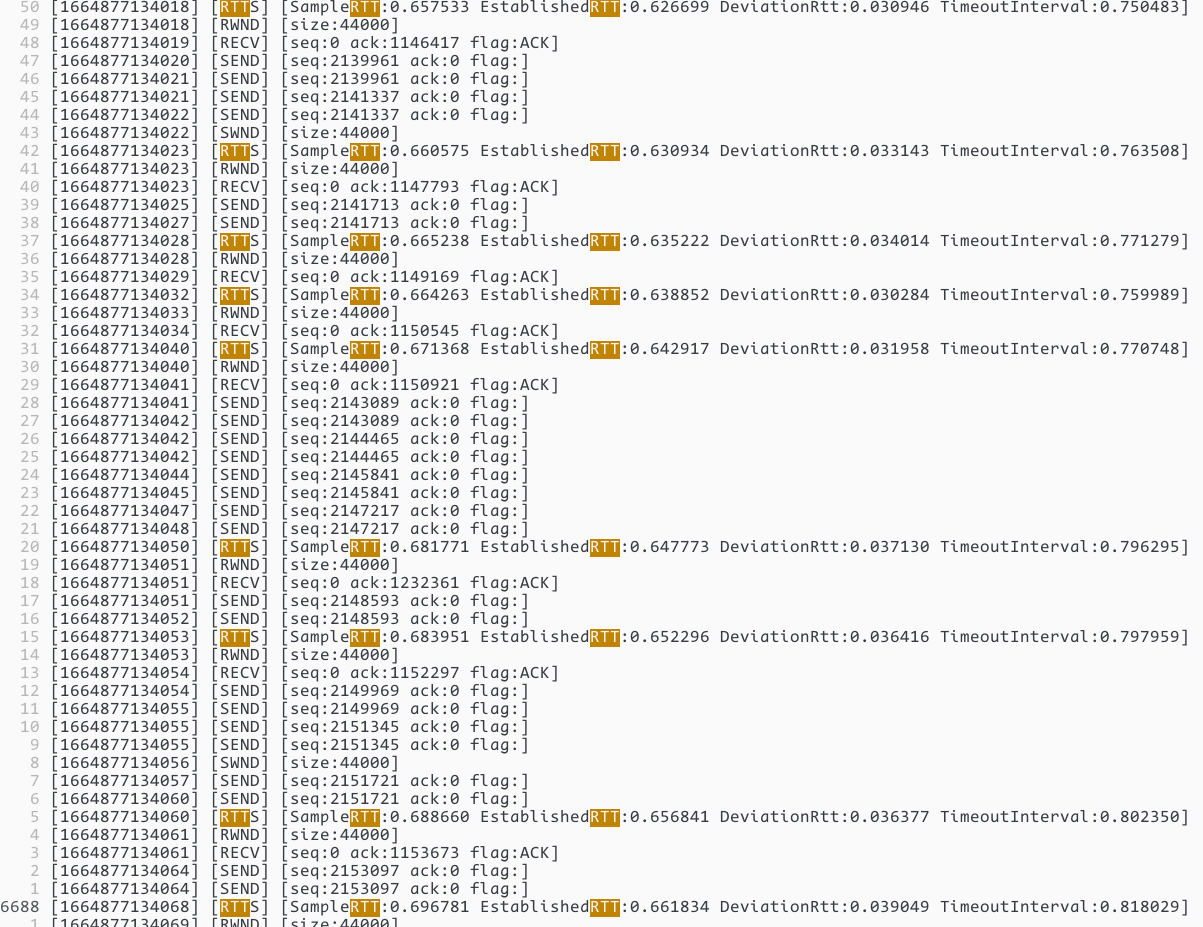
\includegraphics[width=5.5in]{RTT_LOG.png}
    \caption{网站测试结果}\label{fig:LOG}
\end{figure}

\section{可靠数据传输}

我们通过 Client 端的 Trace 可以看到接受到连续 ACK 表明接收到了正确的信息。
\begin{figure}[!htbp]
    \centering
    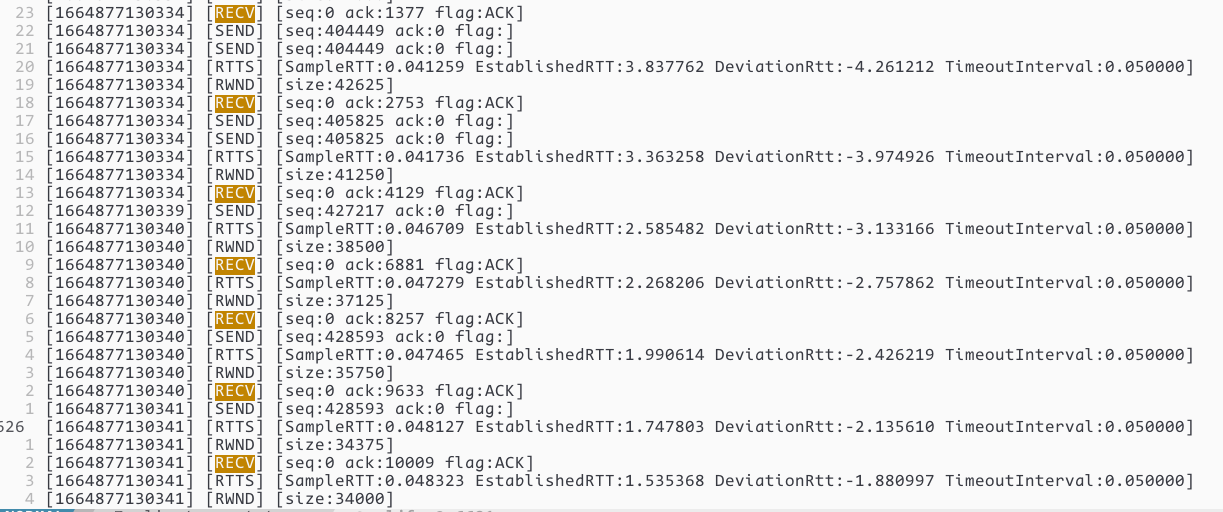
\includegraphics[width=5.5in]{RECV_LOG.png}
    \caption{网站测试结果}\label{fig:recvLog}
\end{figure}

\section{流量控制}
该部分由于系统原因,暂时无法运行提供脚本正确生成图像,将在下周的进度报告中进行补充说明。


\section{AutoLab 测试}
\begin{figure}[!htbp]
    \centering
    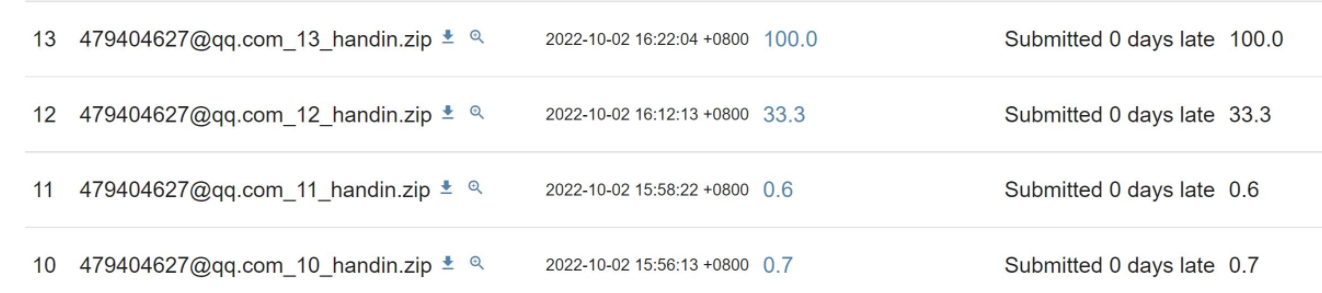
\includegraphics[width=5.5in]{RESULT_WEEK2.png}
    \caption{网站测试结果}\label{fig:net_test}
\end{figure}


\section{人员分工}

人员分工如表\ref{tab:fengong}所示。

\begin{longtable}{p{4em} p{14em}}
    \hline
    人员 & \multicolumn{1}{c}{项目分工} \\
    \midrule
        程子姝 & 完成大部分代码工作,以及协议实现部分 \\ \hline        
        刘锦帆 & 完成 client 和 server 端的处理和 debug.h 以及写作 \\ 
        \hline
    
      \caption{人员分工表}  \label{tab:fengong}
\end{longtable}


